% Options for packages loaded elsewhere
\PassOptionsToPackage{unicode}{hyperref}
\PassOptionsToPackage{hyphens}{url}
%
\documentclass[
  ignorenonframetext,
]{beamer}
\title{Interim Presentation: Renewable Energies}
\author{Jan Besler, Yvette Bodry, Marvin Hoberg, Felix Schulz}
\date{December 16, 2022}

\usepackage{pgfpages}
\setbeamertemplate{caption}[numbered]
\setbeamertemplate{caption label separator}{: }
\setbeamercolor{caption name}{fg=normal text.fg}
\beamertemplatenavigationsymbolsempty
% Prevent slide breaks in the middle of a paragraph
\widowpenalties 1 10000
\raggedbottom
\setbeamertemplate{part page}{
  \centering
  \begin{beamercolorbox}[sep=16pt,center]{part title}
    \usebeamerfont{part title}\insertpart\par
  \end{beamercolorbox}
}
\setbeamertemplate{section page}{
  \centering
  \begin{beamercolorbox}[sep=12pt,center]{part title}
    \usebeamerfont{section title}\insertsection\par
  \end{beamercolorbox}
}
\setbeamertemplate{subsection page}{
  \centering
  \begin{beamercolorbox}[sep=8pt,center]{part title}
    \usebeamerfont{subsection title}\insertsubsection\par
  \end{beamercolorbox}
}
\AtBeginPart{
  \frame{\partpage}
}
\AtBeginSection{
  \ifbibliography
  \else
    \frame{\sectionpage}
  \fi
}
\AtBeginSubsection{
  \frame{\subsectionpage}
}
\usepackage{amsmath,amssymb}
\usepackage{lmodern}
\usepackage{iftex}
\ifPDFTeX
  \usepackage[T1]{fontenc}
  \usepackage[utf8]{inputenc}
  \usepackage{textcomp} % provide euro and other symbols
\else % if luatex or xetex
  \usepackage{unicode-math}
  \defaultfontfeatures{Scale=MatchLowercase}
  \defaultfontfeatures[\rmfamily]{Ligatures=TeX,Scale=1}
\fi
\usetheme[]{Luebeck}
\usecolortheme{whale}
\usefonttheme{structurebold}
% Use upquote if available, for straight quotes in verbatim environments
\IfFileExists{upquote.sty}{\usepackage{upquote}}{}
\IfFileExists{microtype.sty}{% use microtype if available
  \usepackage[]{microtype}
  \UseMicrotypeSet[protrusion]{basicmath} % disable protrusion for tt fonts
}{}
\makeatletter
\@ifundefined{KOMAClassName}{% if non-KOMA class
  \IfFileExists{parskip.sty}{%
    \usepackage{parskip}
  }{% else
    \setlength{\parindent}{0pt}
    \setlength{\parskip}{6pt plus 2pt minus 1pt}}
}{% if KOMA class
  \KOMAoptions{parskip=half}}
\makeatother
\usepackage{xcolor}
\IfFileExists{xurl.sty}{\usepackage{xurl}}{} % add URL line breaks if available
\IfFileExists{bookmark.sty}{\usepackage{bookmark}}{\usepackage{hyperref}}
\hypersetup{
  pdftitle={Interim Presentation: Renewable Energies},
  pdfauthor={Jan Besler, Yvette Bodry, Marvin Hoberg, Felix Schulz},
  hidelinks,
  pdfcreator={LaTeX via pandoc}}
\urlstyle{same} % disable monospaced font for URLs
\newif\ifbibliography
\setlength{\emergencystretch}{3em} % prevent overfull lines
\providecommand{\tightlist}{%
  \setlength{\itemsep}{0pt}\setlength{\parskip}{0pt}}
\setcounter{secnumdepth}{-\maxdimen} % remove section numbering
\usepackage{enumerate}
\ifLuaTeX
  \usepackage{selnolig}  % disable illegal ligatures
\fi

\begin{document}
\frame{\titlepage}

\begin{frame}[allowframebreaks]
  \tableofcontents[hideallsubsections]
\end{frame}
\hypertarget{motivation}{%
\section{Motivation}\label{motivation}}

\begin{frame}{General idea}
\protect\hypertarget{general-idea}{}
Find wasted potential for renewable energies.

\begin{itemize}

\item Illustrate potentials for renewable energies in a user-friendly way
\begin{itemize}
\item Online application as information desk for municipalities and citizens
\item Alternative to complex expert reports
\end{itemize}

\end{itemize}
\end{frame}

\begin{frame}{General idea}
\protect\hypertarget{general-idea-1}{}
We are interested in the expansion of solar power and would like to find
suitable areas for this purpose. Suitable areas are unused spaces that
are not essential for nature or agriculture.

Primary focus: ``Ears'' shaped from highway slip roads.

\begin{figure}
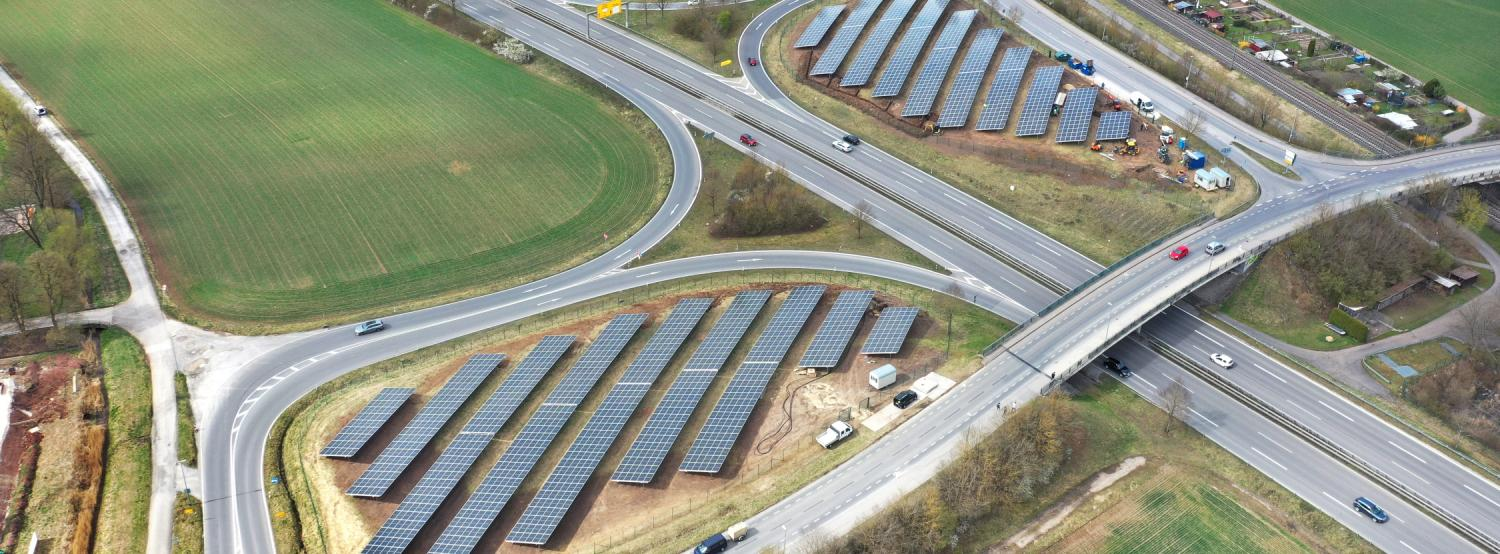
\includegraphics[width=0.85\linewidth]{/Users/Yvette_1/Documents/02-Studium/MSc-Data_Science/2022-23-WS-DS_Project/ds_project/presentations/fig/lustnauer_ohren} \caption{Solar Park Lustnauer Ohren}\label{fig:unnamed-chunk-2}
\end{figure}
\end{frame}

\begin{frame}{General idea}
\protect\hypertarget{general-idea-2}{}
Our contribution:

\begin{itemize}
\item Assess economic utilisation of the identified unused spaces
\begin{itemize}
\item Construction costs vs. Electricity feed
\end{itemize}
\item Assess scalability of idea
\item Tangibility of the general idea
\end{itemize}
\end{frame}

\hypertarget{plan}{%
\section{Plan}\label{plan}}

\begin{frame}{Plan}
\protect\hypertarget{plan-1}{}
\begin{enumerate}
\item Collect geo data
\item Identify "ears" accross Germany
\begin{itemize}
\item Evaluate the suitability of these "ears" for PV
\item Project core: Land cover classification using a neural network:
\begin{enumerate}
\item Other usage: the area has already been built on
\item Added cost: the area is overgrown (trees, bushes, ...)
\item Ideal: Vacant meadow area
\item ...
\end{enumerate}
\end{itemize}
\end{enumerate}
\end{frame}

\begin{frame}{Plan}
\protect\hypertarget{plan-2}{}
\begin{enumerate}[3]
\item Combine neural network results with geographical and meteorological data
\begin{itemize}
\item Distance to grid
\item Meteorological details: Sunshine hours 
\item Sky alignment of the road
\item Geographical details: Ground conditions and slope
\end{itemize}
\end{enumerate}
\end{frame}

\hypertarget{data}{%
\section{Data}\label{data}}

\begin{frame}{Data acquisition: Geo Data}
\protect\hypertarget{data-acquisition-geo-data}{}
As a starting point we choose \textbf{Brandenburg}

\begin{itemize}
\item OpenStreetMap: Street map data in which driveways are clearly identified 
\item Geoportal.de: Aerial images %(data from land surveying offices must be made publically available as of 2019)
  \begin{itemize}
    \item Individual requests revealed cost barriers in three states
    \item Use the coordinates of driveways as filter for downloading relevant images
  \end{itemize}
\end{itemize}
\end{frame}

\begin{frame}{Data on Motorway Slip Roads}
\protect\hypertarget{data-on-motorway-slip-roads}{}
\begin{figure}
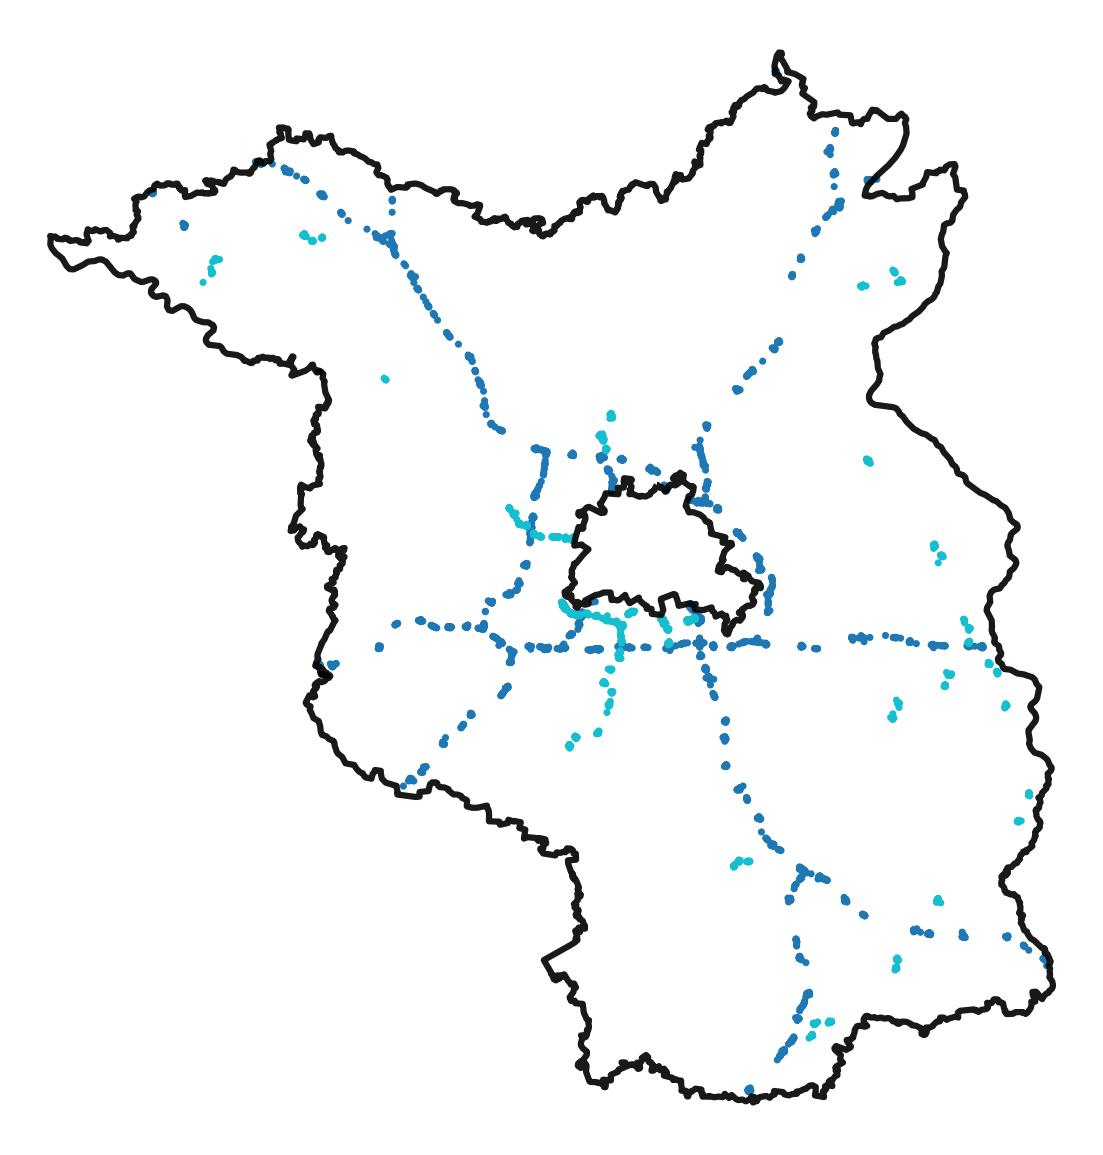
\includegraphics[width=0.33\linewidth]{/Users/Yvette_1/Documents/02-Studium/MSc-Data_Science/2022-23-WS-DS_Project/ds_project/presentations/fig/brandenburg_driveways} \caption{Motorway Slip Roads in Brandenburg}\label{fig:unnamed-chunk-3}
\end{figure}
\end{frame}

\begin{frame}{Data preparation/validation}
\protect\hypertarget{data-preparationvalidation}{}
\begin{figure}

\includegraphics[width = .18\textwidth]{here::here('presentations/fig/driveways_example_1.jpg')}
\vline
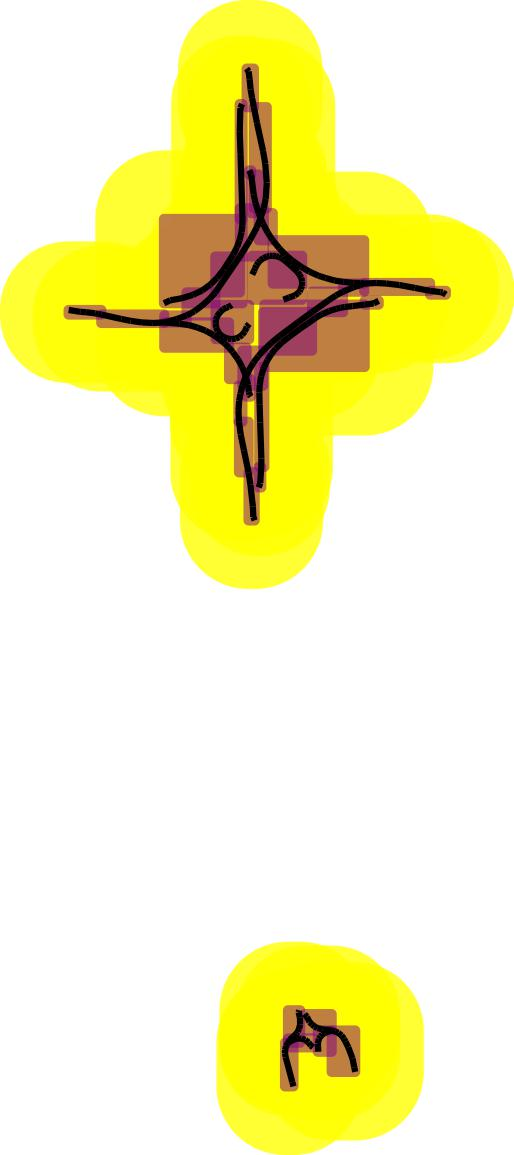
\includegraphics[width = .18\textwidth]{here::here('presentations/fig/driveways_example_2.jpg')}
\vline
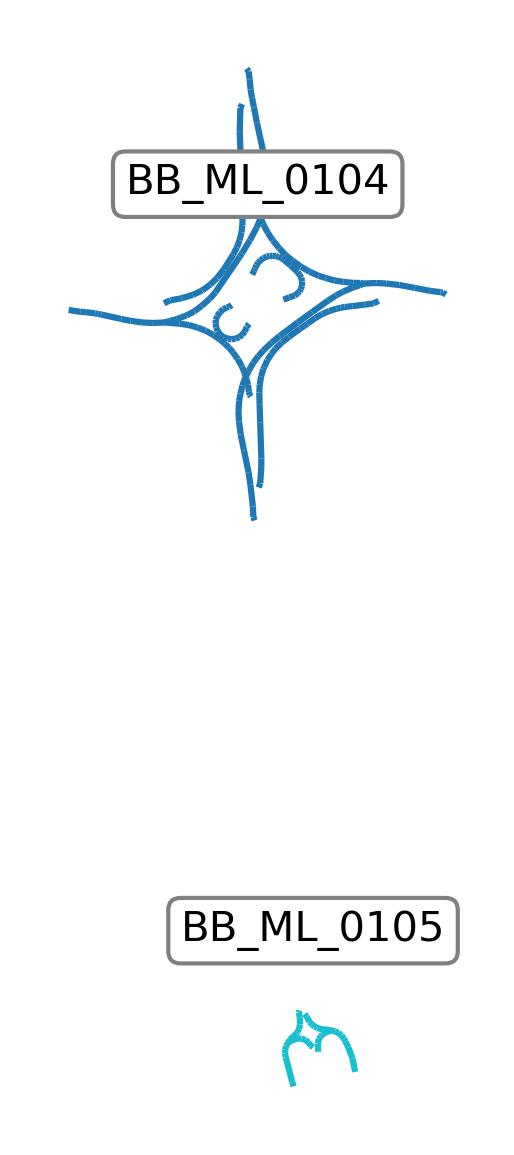
\includegraphics[width = .18\textwidth]{here::here('presentations/fig/driveways_example_3.jpg')}
\vline
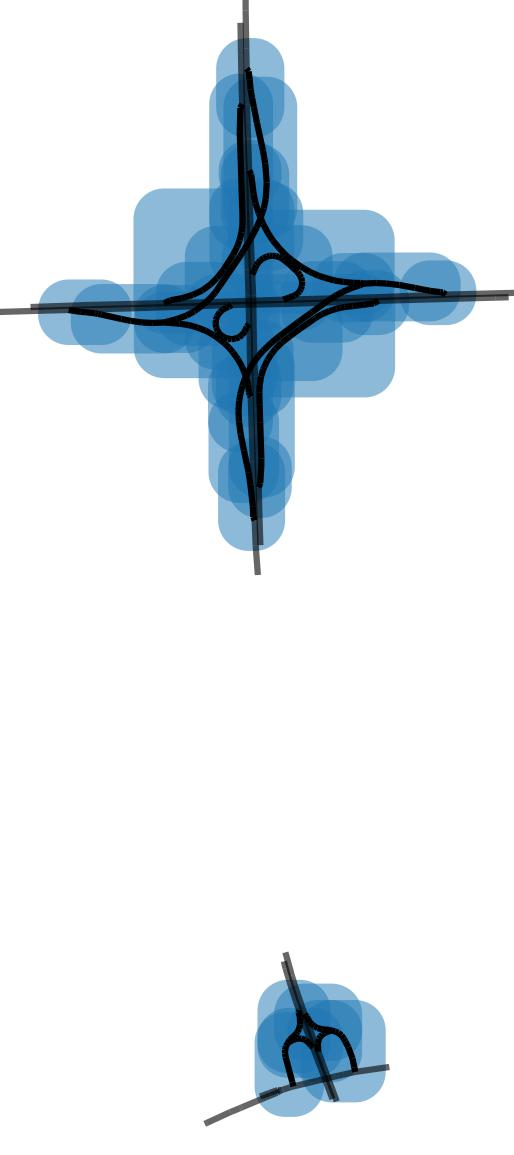
\includegraphics[width = .18\textwidth]{here::here('presentations/fig/driveways_example_4.jpg')}
\vline

\includegraphics[width = .18\textwidth]{here::here('presentations/fig/driveways_example_5.jpg')}
\caption{Example of preprocessing: Matching and IDs}
\end{figure}
\end{frame}

\begin{frame}{Data preparation/validation}
\protect\hypertarget{data-preparationvalidation-1}{}
\begin{figure}
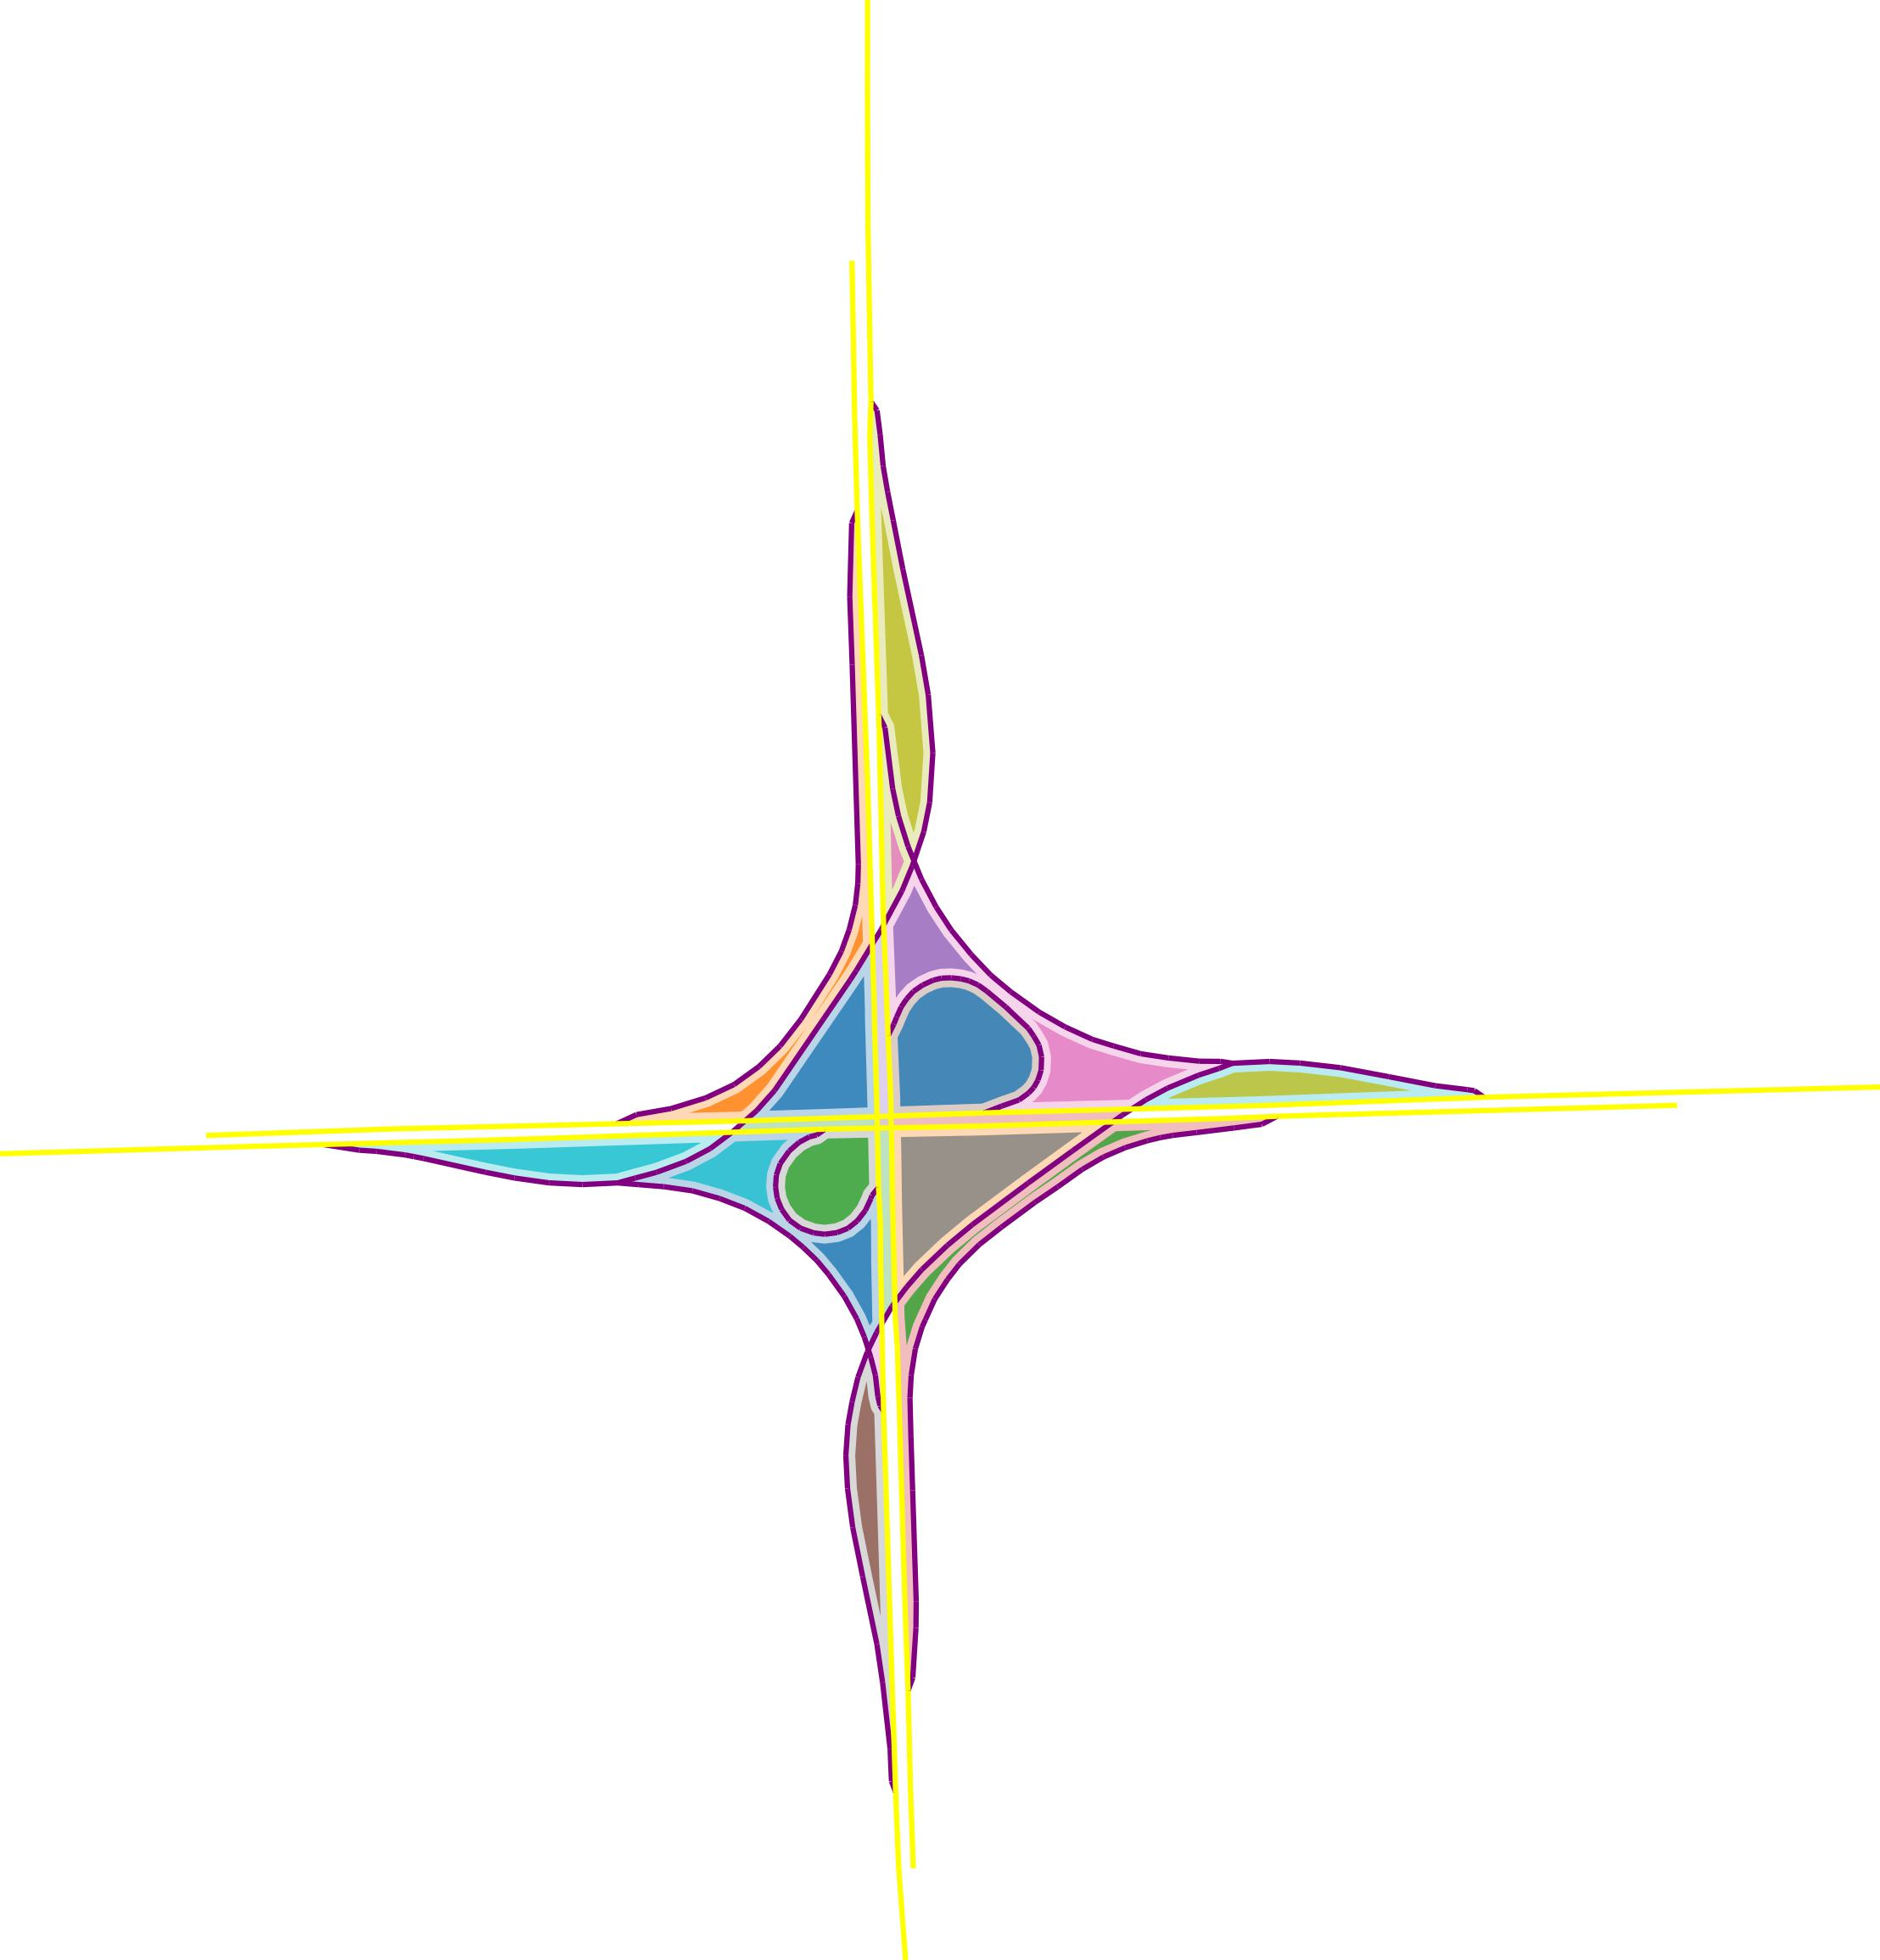
\includegraphics[width = .45\textwidth]{here::here('presentations/fig/driveways_example_6.jpg')}
\hspace{1pt} \vline \hspace{1pt}
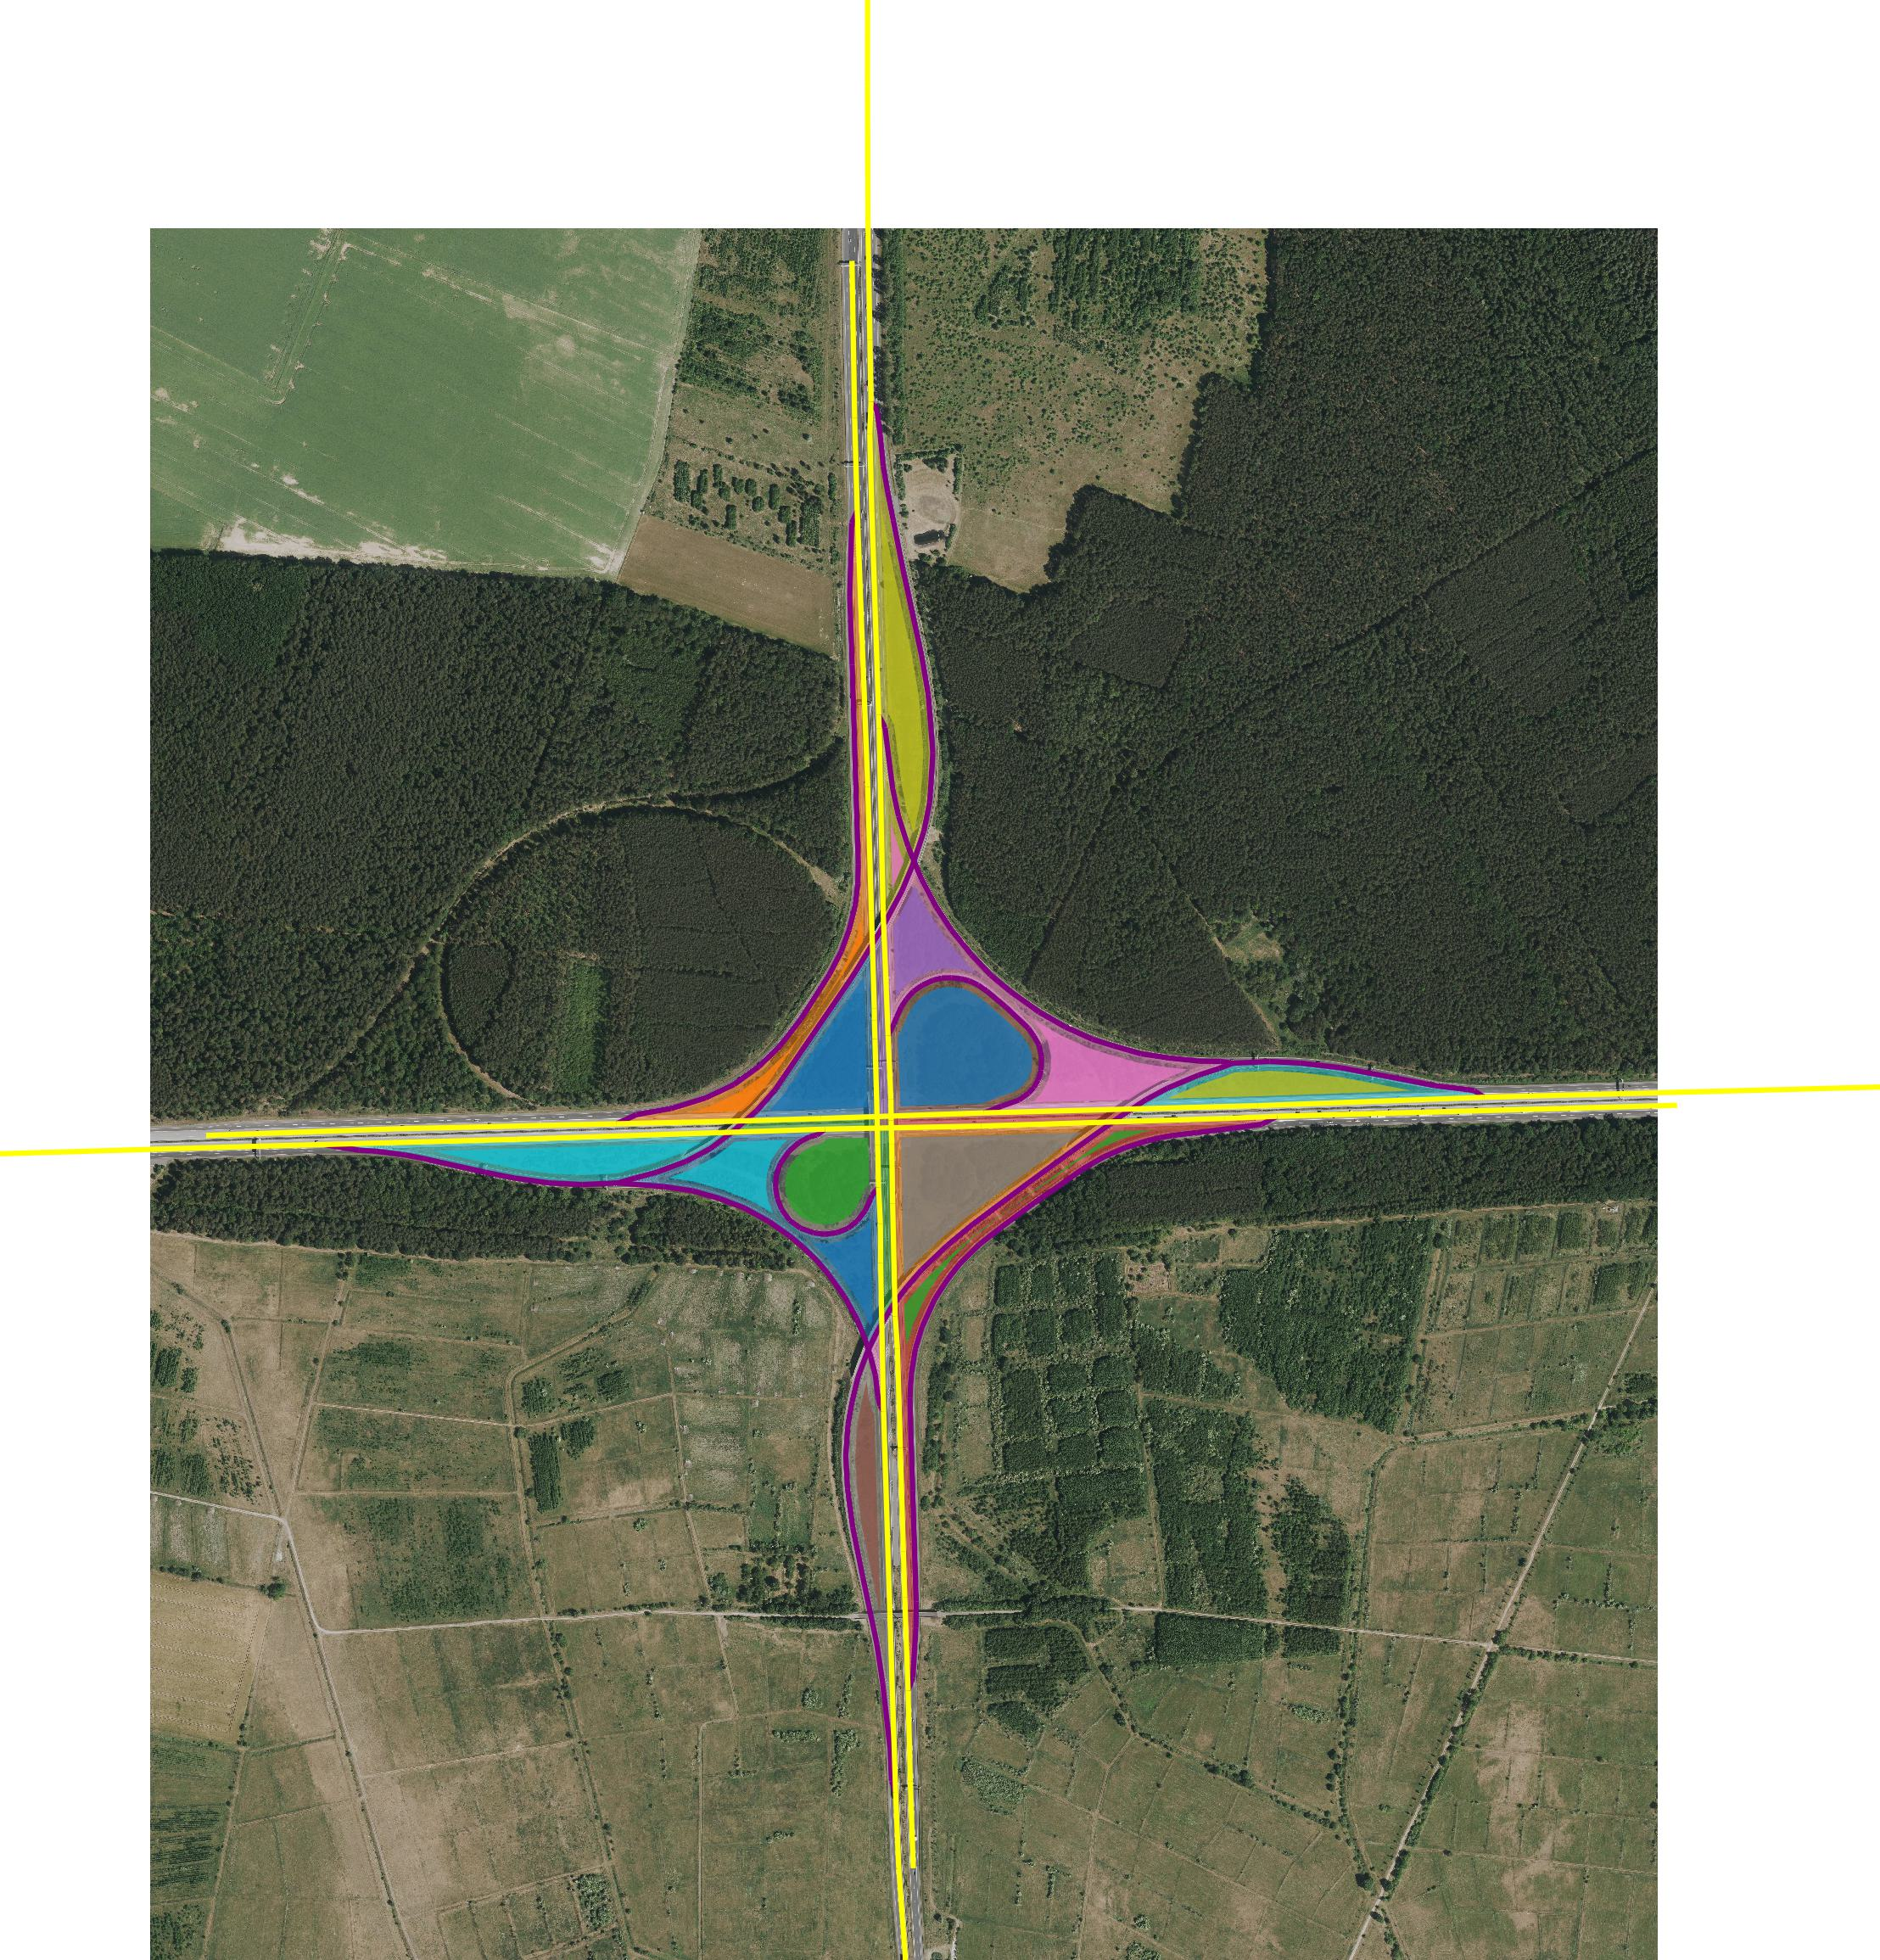
\includegraphics[width = .45\textwidth]{here::here('presentations/fig/driveways_example_7.jpg')}
\caption{Example of preprocessing: Polygons and Imagery}
\end{figure}
\end{frame}

\begin{frame}{Data preparation/validation Pipeline}
\protect\hypertarget{data-preparationvalidation-pipeline}{}
\begin{figure}
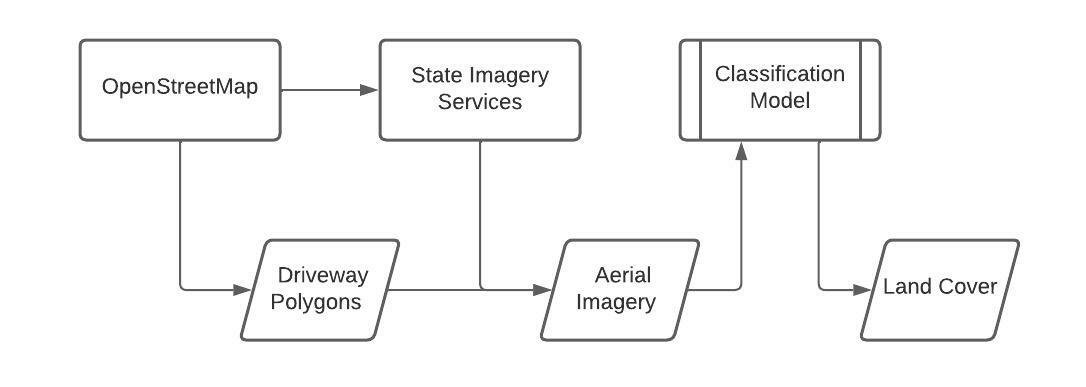
\includegraphics[width=1\linewidth]{/Users/Yvette_1/Documents/02-Studium/MSc-Data_Science/2022-23-WS-DS_Project/ds_project/presentations/fig/ml_pipeline} \caption{The Driveway Data Pipeline}\label{fig:unnamed-chunk-4}
\end{figure}
\end{frame}

\begin{frame}{Economic Model: Geographical and Meteorological Data}
\protect\hypertarget{economic-model-geographical-and-meteorological-data}{}
Further evaluate identified candidate areas for renewable energies with:

\begin{itemize}
\item MaStR: Grid centrality (difficulty of connecting identified zones to existing grid)
\item German Meteorological Service: Sunshine hours (incl. cloud coverage and season)
\item SRTM: Topographical data
\end{itemize}
\end{frame}

\begin{frame}{Economic Model}
\protect\hypertarget{economic-model}{}
\begin{figure}
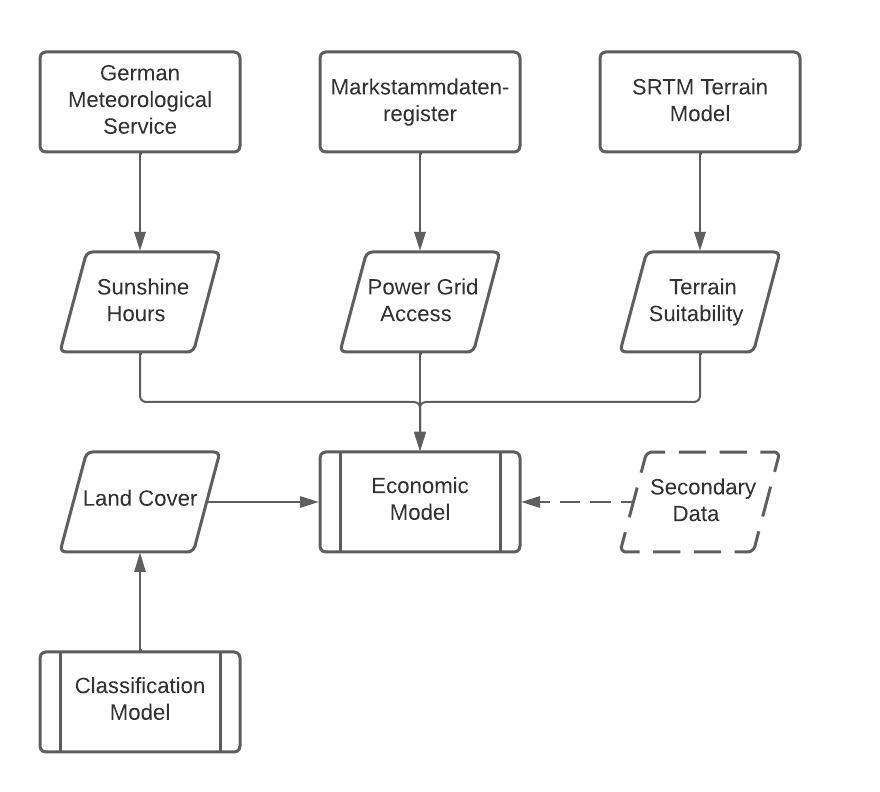
\includegraphics[width=0.6\linewidth]{/Users/Yvette_1/Documents/02-Studium/MSc-Data_Science/2022-23-WS-DS_Project/ds_project/presentations/fig/economic_model} \caption{The Economic Model in Summary}\label{fig:unnamed-chunk-5}
\end{figure}
\end{frame}

\begin{frame}{Data analysis}
\protect\hypertarget{data-analysis}{}
TO DO: Marvin \& Yvette (Trainingsdaten und ResNet)

Easy solution: Pre-trained Convolutional Neural Network (CNN) Two-step
identification (Boxes + Sequencing of relevant shapes) Harder solution:
Self-trained Convolutional Neural Network (CNN) Pixel-specific
identification with data from competition
\end{frame}

\begin{frame}{Data visualization}
\protect\hypertarget{data-visualization}{}
TO DO: Jan htlm

Map with identified ``ears''

Requirements:

\begin{itemize}
\item Location of ears in a selected area
\item Heat map: Colour code for suitability of ears (rating)
\item Features: Size of ear, classification of land coverage, solar hours, grid centrality, ...
\end{itemize}
\end{frame}

\hypertarget{outlook-questions}{%
\section{Outlook/ Questions}\label{outlook-questions}}

\begin{frame}{Outlook/ Questions}
Any experience with landcover classification (remote sensing, image
pixel level) based on a pre-trained neural network?

\begin{itemize}
\item Reference database for neural networks on this objective?
\item Access to pre-trained neural networks free of charge?
\end{itemize}
\end{frame}

\end{document}
